\documentclass{article}

% if you need to pass options to natbib, use, e.g.: \PassOptionsToPackage{numbers, compress}{natbib}
% before loading nips_2016
% to avoid loading the natbib package, add option nonatbib: \usepackage[nonatbib]{nips_2016}

\PassOptionsToPackage{numbers, compress}{natbib}
\usepackage{nips_2016}

% to compile a camera-ready version, add the [final] option, e.g.:
%\usepackage[final]{nips_2016}

\usepackage[utf8]{inputenc} % allow utf-8 input
\usepackage[T1]{fontenc}    % use 8-bit T1 fonts
\usepackage{hyperref}       % hyperlinks
\usepackage{url}            % simple URL typesetting
\usepackage{booktabs}       % professional-quality tables
\usepackage{amsfonts}       % blackboard math symbols
\usepackage{nicefrac}       % compact symbols for 1/2, etc.
\usepackage{microtype}      % microtypography

\usepackage{amsmath,amsthm,color,graphicx,verbatim,listings}
\graphicspath{{figures/}}

\lstset{
numbers=left, 
numberstyle=\small, 
numbersep=8pt, 
frame = single, 
language=matlab, 
framexleftmargin=20pt}

\newtheorem{lemma}{Lemma}

\title{Fast Mini-Batch MCMC for Big Data Bayesian Posterior Inference}

% The \author macro works with any number of authors. There are two commands used to separate the
% names and addresses of multiple authors: \And and \AND.
%
% Using \And between authors leaves it to LaTeX to determine where to break the lines. Using \AND
% forces a line break at that point. So, if LaTeX puts 3 of 4 authors names on the first line, and
% the last on the second line, try using \AND instead of \And before the third author name.

\author{
  David S.~Hippocampus\thanks{Use footnote for providing further
    information about author (webpage, alternative
    address)---\emph{not} for acknowledging funding agencies.} \\
  Department of Computer Science\\
  Cranberry-Lemon University\\
  Pittsburgh, PA 15213 \\
  \texttt{hippo@cs.cranberry-lemon.edu} \\
  %% examples of more authors
  %% \And
  %% Coauthor \\
  %% Affiliation \\
  %% Address \\
  %% \texttt{email} \\
  %% \AND
  %% Coauthor \\
  %% Affiliation \\
  %% Address \\
  %% \texttt{email} \\
  %% \And
  %% Coauthor \\
  %% Affiliation \\
  %% Address \\
  %% \texttt{email} \\
  %% \And
  %% Coauthor \\
  %% Affiliation \\
  %% Address \\
  %% \texttt{email} \\
}

\begin{document}
% \nipsfinalcopy is no longer used

\maketitle

\begin{abstract}
Markov chain Monte Carlo (MCMC) methods have become one of the most popular techniques in machine
learning, but they can be intractably slow when doing Bayesian posterior estimation due to the need
to use information from all training data points during each sampling iteration. We propose a
mini-batch approach that uses information from a small subset of samples per iteration. This, along
with a new Metropolis-Hastings test, will allow us to sample faster to obtain higher-quality
parameter estimates. We implement our sampler in BIDMach and benchmark it with the state of the art.
{\color{blue} Daniel: I hope we can do this.}
{\color{blue} Xinlei: Compare with "cutting MH test budget" paper?}
\end{abstract}

\section{Introduction}

MCMC has become one of the most popular techniques in machine learning...

In this paper, we resolve these challenges\footnote{{\color{blue} Daniel: we can write these
``challenges'' later once the project becomes clearer}.} by proposing an MCMC algorithm for
Bayesian parameter estimation in which proposals are fast and mini-batch based. Our M-H test
acceptance probability is about 50 percent, reasonably high, which means our samples mix well.We
experimentally show that our approach is better than the state of the art.

{\color{blue} Daniel: we can fill out this section later.}

\section{Related Work}

In this section, we review different results on improving MCMC methods with a focus on those dealing
with mini-batches of large datasets. 

Cutting the Metropolis-Hastings Budget paper \cite{ cutting_mh_2014} proposed that there is a bias-variance trade-off in standard MCMC methods. Bias occurs when sampling from the wrong distribution, however, bias usually decreases fast. Variance occurs when the number of sampling is not enough since we can collect only a limited number of samples in a given amount of time. The recently proposed Stochastic Gradient Langevin Dynamics (SGLD) \cite{langevin_2011} and Stochastic Gradient Fisher Scoring methods are biased because they omit the required Metropolis-Hastings tests.


Hamiltonian Monte Carlo (HMC) methods attempt to simulate the ``physics'' of the
system\footnote{Intuitively, we can think of a probability distribution as being a distribution over
particles in the system, where particles are the values of random variables.} in order to generate
distant, high-quality sample proposals (those are the best kind of samples). Since they simulate the
physical dynamics of the system, total energy is preserved and their proposals are always
accepted and there is no need for a Metropolis-Hastings correction/test\footnote{I'm not sure why
this follows but I haven't read the details.}. Unfortunately, HMC methods require the use of a
gradient computation based on all of the data per iteration. (This means the advantage of HMC
methods is that they generate high-quality proposals that mix well; their downside is that they are
unsuitable for big data, which might involve Bayesian posterior inference over that data.)

The Stochastic Gradient Hamiltonian Monte Carlo (SGHMC) method~
\cite{sghmc_2014} tries to compromise
by using a \emph{mini-batch version} of HMC, so each iteration, only the mini-batch is used to
compute the gradient.  SGHMC also includes an extra friction term to counteract the effect of noise
on the system (or gradient) that is added due to using only a small subset of data. (The ``naive''
way of replacing the batch with the mini-batch \emph{without} friction means the system deviates
from the target/desired distribution.) ~\cite{sghmc_2014} assumes the injected noise is Gaussian (we
make a similar assumption) and appeals to the Central Limit Theorem and second-order Langevin
dynamics\footnote{There is a class of MCMC method techniques called \emph{Langevin dynamics}~\cite{mcmc_hamiltonian_2010}. Those algorithms involve computing a gradient update for the parameter of interest $\theta$ and then using the updated $\theta$ as the next sample (i.e., this is like the proposal test). Moreover, by simulating the Hamiltonian dynamics of the system, there is no need for a rejection test. To converge to a \emph{full (posterior) distribution} of $\theta$ and not a single point (i.e., the MAP estimate of $\theta$, or the mode of the distribution) langevin dynamics adds Gaussian noise each iteration to cause the $\theta$ samples to ``jump around.'' The work of~\cite{langevin_2011} is closer to ours because it applies the normal Langevin dynamics algorithm with one difference: the gradient updates are based on a \emph{mini-batch} of the original data.} to show that SGHMC maintains the desired target distribution as the stationary
distribution. Our methods are similar in that we use mini-batches of data, but the difference is
that they focus on improving a particular flavor of MCMC, \emph{Hamiltonian} Monte Carlo (which uses Langevin dynamics to add noise), and they
also try avoiding MH tests, while we are focused on improving \emph{general} MCMC by means of a \emph{more efficient} MH proposal. These are different ways of solving the same problem (i.e., the problem of using mini-batches of
large data for MCMC).

The work of~\cite{cutting_mh_2014} also concerns speeding up MCMC 
by using mini-batches of data. Their argument is that the standard MCMC algorithm for Bayesian
posterior inference (i.e., to compute $p(\theta \mid x_1, \ldots, x_N)$ for i.i.d. data points) is
unsuitable for large datasets because the likelihood computation requires the use of all points,
$p(x_1, \ldots, x_n \mid \theta) = \prod_{i=1}^Np(x_i\mid \theta)$. Using all of this data just to
decide whether the new sample $\theta$ should be accepted or rejected is computationally
inefficient. In theory, given infinite time, using all the data points is fine because it results in
an unbiased estimate of the target distribution and the variance of the resulting sampled values is
low given enough time.\footnote{Note that~\cite{cutting_mh_2014} primarily use MCMC to estimate just
the expectation of the target distribution, but their analysis should extend to other values of the
target distribution for arbitrary input $\theta$. In other words, they use MCMC to estimate
$\mathbb{E}[p(\theta \mid x_1, \ldots, x_N)]$, but we are mostly interested in $p(\theta \mid x_1,
\ldots, x_N)$.} In reality, we have limited time. The key argument in~\cite{cutting_mh_2014} is that
given a fixed budget, it may be better to use $n$ data points per iteration (where $n \ll N$), which
will sacrifice some bias but will perhaps improve variance by allowing us to sample for $\theta$
more often, since we will get $\theta_1, \ldots, \theta_T$ as opposed to the standard case using all
$N$ samples but with only $\theta_1, \ldots, \theta_t$ samples ($t \ll T$).

More formally, the algorithm they develop is a sequential hypothesis testing algorithm. During each
iteration, their algorithm generates a new sample $\theta'$ from the proposal distribution. They
start with a small mini-batch of the data, and test the hypothesis (based on this small mini-batch)
that $\theta'$ should be accepted or rejected based the likelihood ratio. (Intuitively, we can
easily tell if $\theta'$ will be accepted/rejected if the mini-batch of data results in likelihood
drastically different from the likelihood of the current sample $\theta$.) If the hypothesis test is
too uncertain, then we increase the mini-batch size and apply the test again, and we repeat this
increment until we accept or reject $\theta'$ with high confidence (based on a Student-t
distribution). The downside of this algorithm is the need to keep incrementing the mini-batch size in one iteration; in the worst case, they may not be able to tell with confidence to accept or
reject until we get nearly all $N$ of the data points, which defeats the purpose of the algorithm.
We propose our own algorithm that avoids this problem. {\color{blue} Daniel: does this make sense as
a ``weakness'' of their approach?  Ideally I would like to have a comparison between our method and
theirs.}

Some additional references to use:

\begin{itemize}
    \item \cite{icml2014c1_bardenet14} (ICML 2014) I think we definitely want to consider this. It
    seems to be ``an alternative to the Cutting the MH budget approach'' and so it might also be
    considered as a direct competitor.
    \item \cite{conf/icml/AhnBW12} (ICML 2012) is the ``successor'' to Stochastic Gradient Langevin
    Dynamics.
    \item \cite{conf/uai/MaclaurinA14} (UAI 2014) seems like it would be interesting to state its
    limitations.
    \item \cite{mcmc_hamiltonian_2010} is a long paper and is written like a chapter in a textbook,
    so it's for pedagogical reasons. It describes MCMC with Hamiltonian dynamics. It is useful to
    gain some background on a lot of the HMC-related papers that have come since its publication
    (2010).
    \item \cite{stochastic_thermostats_2014} (NIPS 2014) might be considered as a ``competitor''
    though only for HMC cases.
    \item \cite{sgmcmc_2015} (NIPS 2015) might want to give this a mention, where it would fit in
    their recipe.
\end{itemize}



\section{Our Algorithm}\label{sec:our_algorithm}

\subsection{The General MCMC Method}\label{sec:general_mcmc}

The general MCMC method proceeds as follows. For a desired random vector $\theta$, we have a
\emph{target distribution} we wish to compute, $p(\theta \mid x_1, \ldots, x_N)$, based on $N$
i.i.d. data points. Since exact evaluation is intractable, we generate a chain of correlated samples
$\theta_1, \ldots, \theta_T$ for some large $T$, and approximate $p$ by using counts of samples. For
each iteration $t$, we start with our current $\theta_t$. We use a \emph{proposal distribution}
$q(\theta' \mid \theta_t)$ to determine a new candidate $\theta'$. With probability $P_a$, we accept
it and set $\theta_{t+1} = \theta'$; otherwise, we repeat the previous value $\theta_{t+1} =
\theta_t$. Traditionally, $P_a$ is computed as follows:
\begin{equation}\label{eq:traditional}
P_a = \min\left\{ 1, \frac{f(\theta')q(\theta_t \mid \theta')}{f(\theta_t)q(\theta' \mid \theta_t)}
\right\} = \min\left\{ 1, \frac{p(\theta')\prod_{i=1}^N p(x_i ; \theta')q(\theta_t \mid \theta')}{p(\theta_t)\prod_{i=1}^N p(x_i ; \theta_t)q(\theta' \mid
\theta_t)} \right\},
\end{equation}
where $f(\theta_t)=p(\theta_t|x_1,\ldots,x_N) \propto p(\theta_t)\prod_{i=1}^N p(x_i
\mid \theta_t)$ which roughly tells us how ``likely'' we are to have a $\theta_t$ sample. The
normalizing constants cancel out, so the requirement for $P_a$ is that $f$ be proportional to the
true target distribution.

One then draws a uniform random variable $u$ from ${\rm Unif}[0,1]$ and accepts $\theta_{t+1} =
\theta'$ if $u < P_a$, and uses $\theta_{t+1} = \theta_t$ otherwise. The $P_a$ from
Equation~\ref{eq:traditional} satisfies ``detailed balance'' which, roughly speaking, means that if
we sample long enough using the heuristic above, we will arrive at a stationary distribution.

The $P_a$ is guaranteed to converge to the true $p$ distribution given sufficiently many examples
(though a burn-in period and/or taking every $n$th sample may be necessary). Unfortunately,
computing $f$ requires the use of all $N$ training data points. In this paper, we derive a new fast,
approximate Metropolis-Hastings test which does not use all $N$ points during each test.

\subsection{A Different Metropolis-Hastings Test}\label{sec:faster}

\begin{figure}[t]
  \centering
  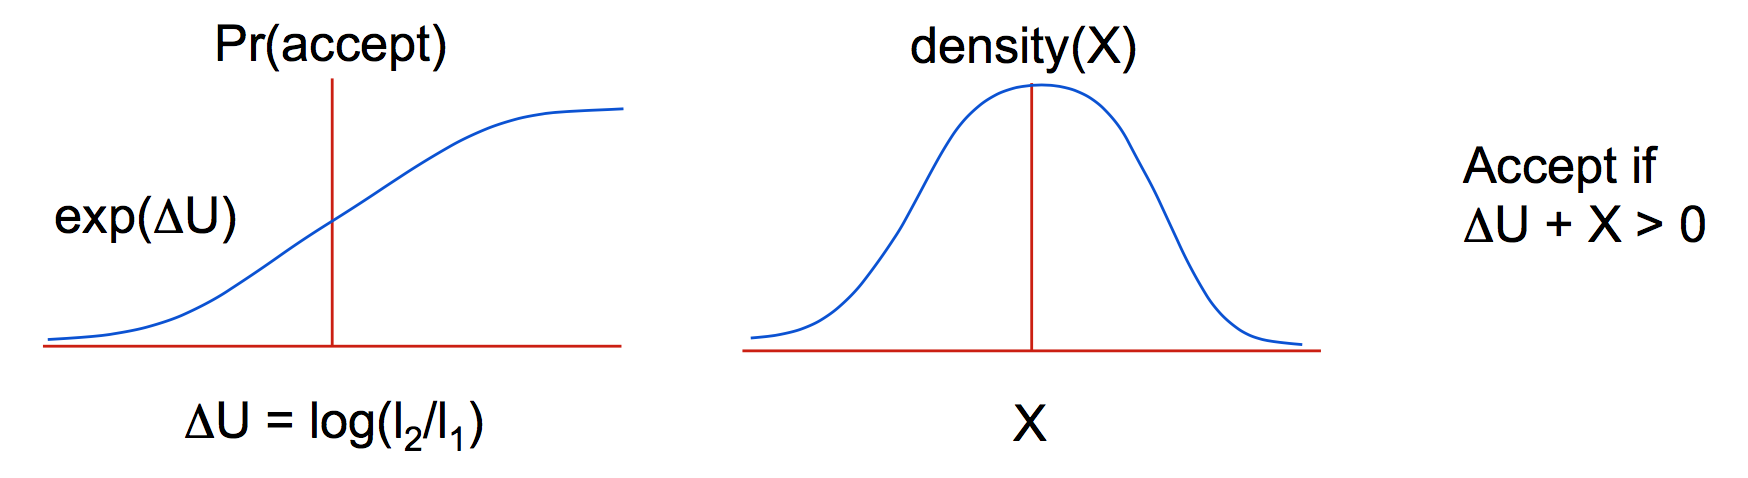
\includegraphics[width=\textwidth]{john_bair_fig01}
  \caption{
  To the left is the logistic distribution, representing a possible acceptance test. As $\Delta U$
  approaches infinity, the acceptance rate approaches 1. To the right, we have a new variable $X$
  and its density, along with an acceptance test $\Delta U + X$, which we describe in detail in
  Section~\ref{sec:our_algorithm} (note that we use $\Delta$ instead of $\Delta U$ for simplicity).
  {\color{blue}
  Daniel: I think that the diagram to the left should use the logistic function, i.e., replace
  ``$\exp(\Delta U)$'' with ``$(1+\exp(\Delta U))^{-1}$.''
  }
  }
  \label{fig:part1}
\end{figure}

\begin{figure}[t]
  \centering
  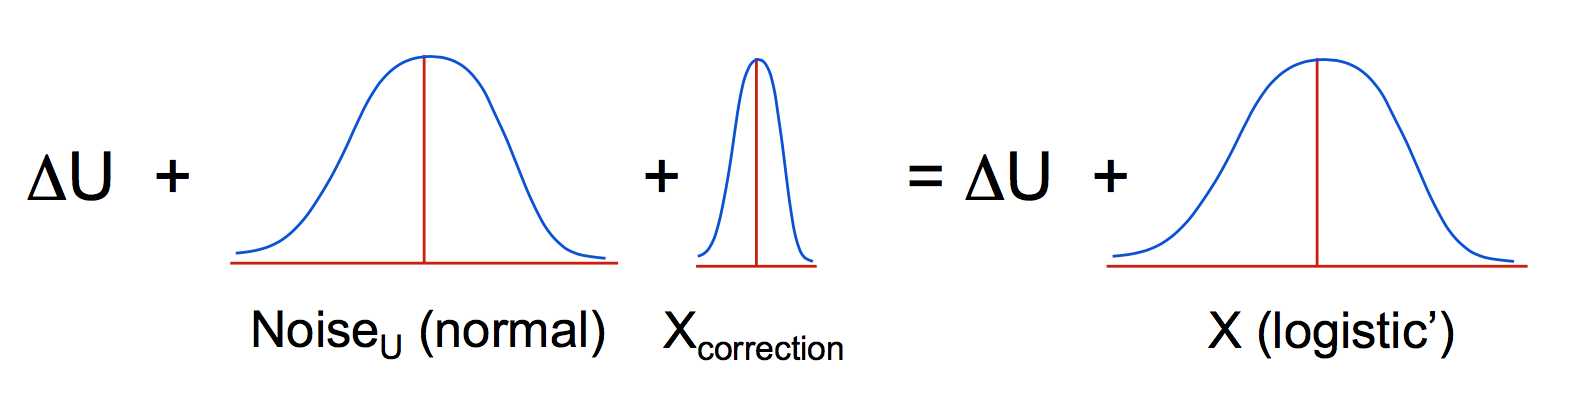
\includegraphics[width=\textwidth]{john_bair_fig02}
  \caption{
  To the left, we have $\Delta U$ (which is simplified as $\Delta$ in
  Section~\ref{sec:our_algorithm}), along with two noise terms that come from the new variable we
  define $X$. The details are in Section~\ref{sec:our_algorithm}.
  }
  \label{fig:part2}
\end{figure}

Our starting point is the following Lemma.

\begin{lemma}\label{lem:detailed_balance}
Let $\Delta = \log \left(\frac{f(\theta') q(\theta_t \mid
\theta')}{f(\theta_t) q(\theta'\mid \theta_t)} \right)$, where $f$ is proportional to the desired target distribution and $q$ is our chosen
proposal distribution. Any acceptance function $g$ such that $g(\Delta) = \exp(\Delta) g(-\Delta )$
satisfies detailed balance. That is, $f(\theta_t)p(\theta' \mid \theta_t) = f(\theta')p(\theta_t
\mid \theta')$, where $p(\theta_y \mid \theta_x)$ is the probability of jumping from $\theta_x$ to $\theta_y$ in our chain.
\end{lemma}

\begin{proof}
We begin by deriving $p(\theta' \mid \theta_t)$. This is equivalent to the probability of proposing
$\theta'$ and then accepting it, so
\begin{equation}\label{eq:one_way}
p(\theta' \mid \theta_t) = q(\theta' \mid \theta_t)g(\Delta).
\end{equation}
Similarly, we have
\begin{equation}\label{eq:other_way}
p(\theta_t \mid \theta') = q(\theta_t \mid \theta')g(-\Delta).
\end{equation}
Notice that the probability of accepting a transition from $\theta'$ to $\theta_t$ is $g(-\Delta)$
because this inverts the fraction inside the logarithm term of $\Delta$.  By assumption, we can
expand $g(\Delta) = \exp(\Delta)g(-\Delta)$ in Equation~\ref{eq:one_way}.  Doing this, and combining
the result of Equation~\ref{eq:other_way}, we get
\begin{equation}\label{eq:combined}
g(-\Delta) = \frac{p(\theta' \mid \theta_t)}{q(\theta' \mid \theta_t)\exp(\Delta)} = \frac{p(\theta_t \mid \theta')}{q(\theta_t \mid \theta')}.
\end{equation}
Rearranging terms and expanding $\exp(\Delta)$, we have
\begin{equation}\label{eq:rearrange}
\frac{p(\theta' \mid \theta_t) f(\theta_t) q(\theta' \mid \theta_t)}{q(\theta' \mid \theta_t) f(\theta') q(\theta_t \mid \theta')} = \frac{p(\theta_t \mid \theta')}{ q(\theta_t \mid \theta')}.
\end{equation}
Cancellations result in $f(\theta') p(\theta_t \mid \theta') = f(\theta_t) p(\theta' \mid \theta_t)$. Thus, detailed balance is satisfied.\\
\end{proof}

Some straightforward arithmetic shows that the standard Metropolis-Hastings acceptance function
$g(\Delta) = \min\{1, e^\Delta \} = \min\left\{1, \frac{f(\theta')q(\theta_t \mid \theta')}{f(\theta_t)q(\theta' \mid
\theta_t)}\right\}$ satisfies the condition $g(\Delta) =
\exp(\Delta)g(-\Delta)$ and consequently, results in detailed balance.

For reasons that will be clear later, we choose an alternative $g$, the logistic function:
$g(\Delta) = (1+\exp(-\Delta))^{-1}$. Again, straightforward arithmetic shows that it satisfies the
condition in Lemma~\ref{lem:detailed_balance}.

We can sample from the logistic function using the following procedure. Let $u$ be drawn from ${\rm
Unif}[0,1]$. At any given iteration, we can compute $\Delta$, and we accept the new candidate
$\theta'$ if $g(\Delta) > u$, and reject otherwise. Let us define the random variable $X =
g^{-1}(u)$ where again, $g$ is the logistic function. We claim that $X$ has CDF function $F_X(x) =
g(x)$, i.e., its CDF is precisely the logistic function. This is because for some $X = x$, we have
\[
F_X(x) = {\rm Pr}(X \le x) = {\rm Pr}(g^{-1}(u) \le x) = {\rm Pr}(u \le g(x)) = \int_{0}^{g(x)} 1 dx = g(x),
\]
as the density of the uniform random variable here is simply one. Thus, the criteria to accept the
candidate $\theta'$ is equivalent to whether $\Delta > X$, where $X$ has CDF of logistic function.
(If this isn't immediately obvious, note that we can pre-multiply $g^{-1}$ to $g(\Delta) \ge u$, and
our test is $\Delta > X$.) Since $X$ is symmetric about zero, the acceptance criteria can also be
expressed as $\Delta + X>0$, as shown in Figure~\ref{fig:part1}.

{\color{blue}
Daniel: The above makes sense, but I still don't understand why we had to show that the CDF of $X$
is the logistic function, because I never use that when I claim that our acceptance test is now
$\Delta > X$.  Do we need that assumption so that, for instance, we can decompose $X$ later the way
we do it, with $X_{\rm noise}$ having the same variance as $\epsilon$? That might explain it.
}

Unfortunately, there's a problem with the $\Delta + X > 0$ test: it requires us to compute $\Delta$,
so our test will be slow! We can get around this by defining a new scalar-valued term, $\Delta'$, which is
computed the same way as $\Delta$, but uses far fewer samples. In other words, $\Delta'$ is computed
based on a \emph{mini-batch} of data, and it is an approximation of $\Delta$, so we can express the
relationship as $\Delta' = \Delta + \epsilon$ for a noise term $\epsilon$. \emph{The key is that
$\epsilon$ follows a normal distribution}, $\epsilon \sim \mathcal{N}(0, \sigma^2)$, because for i.i.d. data $x_1, \ldots, x_N$, the $\Delta$
is expressed as the sum of log probabilities (look at Equation~\ref{eq:traditional} and apply the
logarithm to the product over the $N$ data points, to get a sum of log terms). All we do with
$\Delta$ is take far fewer of the summations, and normally-distributed noise is there as a product
of the Central Limit Theorem.

To sample accurately from $\Delta'$, we need to slightly change our acceptance criteria. We can
decompose $X$ as $X = X_{\rm norm} +X_{\rm correction}$, where the first term is a ``noise term''
which has the same variance as $\epsilon$, and the second term is a ``residual'' term. The criteria
to accept, previously expressed as $\Delta + X > 0$, can be rewritten as
\begin{equation}\label{eq:criteria}
\Delta + X = \Delta + X_{\rm norm} + X_{\rm correction} \approx \Delta' + X_{\rm correction} >0.
\end{equation}
This explains Figure~\ref{fig:part2} (though it really should be an approximation as we can't guarantee that our $X_{\rm norm}$ term is exactly the correct amount of noise), where the left hand side has distributions representing normal
noise ($X_{\rm norm}$, which is labeled as ${\rm Noise}_U$, but they are the same thing) and a
``correction'' term labeled $X_{\rm correction}$. Be aware that all of these ``additions'' are to be
interpreted as convolutions when computing the sum of densities.

Notice that we have several options we can control. For instance, we can adjust the mini-batch size;
increasing the mini-batch size will cause the $X_{\rm noise}$ distribution to shrink and become
narrower.

{\color{blue} Daniel: I think it's becoming clear but I'm still trying to connect all of the steps.
During each iteration of MCMC, we compute $\Delta'$ and \emph{sample} (right?) an $X$ (which we can
do by sampling $u$ and then doing $X = g^{-1}(u)$. This gives us $\Delta' + X$ but our MH test
    actually requires $X_{\rm correction}$, so first we must estimate $\sigma^2$, the variance of
    $X_{\rm noise} \sim \mathcal{N}(0, \sigma^2)$ (perhaps from the mini-batch data, somehow?) and
    then somehow ``remove'' that component from $X$ to get $X_{\rm correction}$? Then we have our
    acceptance test. Is this right? Or, of course, we don't have to sample $X$ at all, but just
    figure out a way to sample $X_{\rm correction}$ directly.

I think we talked about estimating $\sigma^2$. The variance $\sigma^2$ that we're concerned about is
a scalar value based on the sum of log probabilities of different samples, so one way we could
estimate the variance is by taking all samples of a mini-batch and seeing how much those individual
$\log p(x_i \mid \theta)$ vary. Or we could look at $k$ mini-batches of data which will give us
$\Delta_1, \ldots, \Delta_k$ and compute the empirical $\sigma^2$ (of course that defeats the
purpose of using mini-batches).  }

{\color{blue} Xinlei: I agree with you that out MH test requires $X_{correction}$. My understanding
is that we can actually estimate $X$ from the whole data set, and the probability distribution of
$X_{norm}$ is what we proposed? So the determination of $X_{correction}$ is a deterministic
deconvolution problem.  }




\section{Implementation}\label{sec:implementation}

We implement our system within the open-source BIDMach project~\cite{canny2013bidmach}. Note to
ourselves: do NOT modify the \texttt{Learner.scala} code -- just make it a new ``Model''.




\section{Experiments}\label{sec:experiments}

\subsection{Experiment 1}

\subsection{Experiment 2}




\section{Conclusion}\label{sec:conclusion}


\small
\bibliography{nips_2016}
\bibliographystyle{ieeetr}

\clearpage
\appendix

\section{Section for Appendix Information}

{\color{blue}
Daniel: In case we want to use this.
}


% Daniel: here are example LaTeX codes for figures and tables if we want to use them.

%\begin{figure}[h]
%  \centering
%  \fbox{\rule[-.5cm]{0cm}{4cm} \rule[-.5cm]{4cm}{0cm}}
%  \caption{Sample figure caption.}
%\end{figure}

%\begin{table}[t]
%  \caption{Sample table title}
%  \label{sample-table}
%  \centering
%  \begin{tabular}{lll}
%    \toprule
%    \multicolumn{2}{c}{Part}                   \\
%    \cmidrule{1-2}
%    Name     & Description     & Size ($\mu$m) \\
%    \midrule
%    Dendrite & Input terminal  & $\sim$100     \\
%    Axon     & Output terminal & $\sim$10      \\
%    Soma     & Cell body       & up to $10^6$  \\
%    \bottomrule
%  \end{tabular}
%\end{table}

%\usepackage[pdftex]{graphicx} ...
%\includegraphics[width=0.8\linewidth]{myfile.pdf}

\end{document}
